\documentclass{article}

%other packages
\usepackage[a4paper]{geometry}
\usepackage{longtable}
\usepackage{wrapfig}
\setlength\parindent{0pt}
\usepackage{enumitem}
\usepackage[table,dvipsnames]{xcolor}
\usepackage{polynom}
\def\scaleint#1{\vcenter{\hbox{\scaleto[3ex]{\displaystyle\int}{#1}}}}
\usepackage{array}
\newcolumntype{C}{>{{}}c<{{}}} % for '+' and '-' symbols
\newcolumntype{R}{>{\displaystyle}r} % automatic display-style math mode 
\usepackage{tabularray}
\usepackage{dcolumn,tabularx,booktabs}
\usepackage[most]{tcolorbox}
%\graphicspath{ {C:/Users/twill/OneDrive/Desktop/Eliason/Diagrams} }

%maths
\usepackage{mathtools}
\usepackage{amsmath}
\usepackage{amssymb}
\usepackage{amsfonts}
\usepackage{autobreak}

%tikzpicture
\usepackage{tikz}
\usepackage{scalerel}
\usepackage{pict2e}
\usepackage{tkz-euclide}
\usepackage{tikz-3dplot}
\usetikzlibrary{calc}
\usetikzlibrary{patterns,arrows.meta}
\usetikzlibrary{shadows}
\usetikzlibrary{external}
\usetikzlibrary{decorations.pathreplacing,angles,quotes}

%pgfplots
\usepackage{pgfplots}
\pgfplotsset{compat=1.18}
\usepgfplotslibrary{statistics}
\usepgfplotslibrary{fillbetween}

\pgfplotsset{
    standard/.style={
    axis line style = thick,
    trig format=deg,
    enlargelimits,
    axis x line=middle,
    axis y line=middle,
    enlarge x limits=0.15,
    enlarge y limits=0.15,
    every axis x label/.style={at={(current axis.right of origin)},anchor=north west},
    every axis y label/.style={at={(current axis.above origin)},anchor=south east}
    }
}

\begin{document}

{\bf{}EXAMPLE} Find the area between the branches of the hyperbola $y^2-x^2=4$ for $0\leq x\leq1$.

\[\Rightarrow y^2=4+x^2=\left\{\begin{aligned}\sqrt{x^2+4}&\quad for\quad y<0\\-\sqrt{x^2+4}&\quad for\quad y\geq0\end{aligned}\right.=\left\{\begin{aligned}x=a\sinh t\\y=a\cosh t\end{aligned}\right.\]

General hyperbola: $y^2/b^2-x^2/a^2=1$

\begin{center}
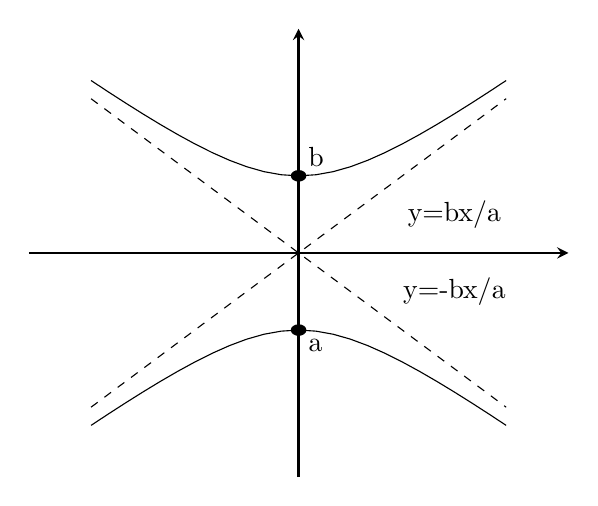
\begin{tikzpicture}
\begin{axis}[standard,domain=-4:4,xtick={\empty},ytick={\empty}]
\addplot[] {(x^2+4)^0.5};
\addplot[] {-(x^2+4)^0.5};
\addplot[dashed] {x};
\fill[] (0,2) circle [radius=0.15] node[above right]{b};
\node[] at (3,1) {y=bx/a};
\addplot[dashed] {-x};
\node[] at (3,-1) {y=-bx/a};
\fill[] (0,-2) circle [radius=0.15] node[below right]{a};
\end{axis}
\end{tikzpicture}
\end{center}


And we could solve this by paramaterizing the equation or using a substitution. Both hyperbolic.

\vspace{10pt}

We are definitely going to be expected to know hyperbolic properties, such as $\sinh2t=2\sinh t\cosh t$. These are similar to their trigonometric counterparts.

\end{document}

